Les s\'eries enti\`eres sont consid\'er\'ees comme des vecteurs et compar\'ees avec une distance qui utilise toutes les valeurs des s\'eries. 
%L'utilisation de toutes les valeurs est exig\'ee parce que les valeurs de chaque s\'erie peuvent \^etre diff\'erente \`a n'importe quel temps.
Cette distance calcule la similarit\'e entre ces deux s\'eries.
La similarit\'e entre deux s\'eries enti\`eres est excellente  s'il existe des caract\'eristiques discriminatoires identiques entre ces s\'eries sur l'axe du temps. Ces caract\'eristiques peuvent \^etre identifi\'ees aux m\^emes instants de temps ou \`a des instants d\'ecal\'es mais constants dans le temps. 
\newline
Par exemple, consid\'erons le dataset {\em FiftyWord} \cite{rath2003word} dans lequel les donn\'ees proviennent de la base de donn\'ee {UCR} \cite{chen2015ucr} et d\'ecrivent les contours des mots \'ecris par Georges Washington dans sa biblioth\`eque priv\'ee. Dans la figure \ref{caracteristiquesFiftyWordUCR}, nous distinguons $4$ s\'eries regroup\'ees en $2$ classes. Les deux s\'eries du haut (en noir) identifient la classe $30$ et les deux s\'eries du bas (en vert) identifient la classe $50$. Le motif commun est observable en alignant les s\'eries.
% ---- figure caracteristiquesFiftyWordUCR.
\begin{figure}[htb!] 
\centering
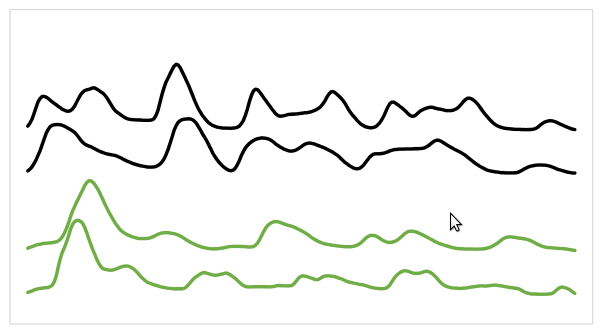
\includegraphics[scale = 0.5]{caracteristiquesFiftyWordUCR.jpeg}
\caption{D\'etection du motif commun en alignant les s\'eries. Les deux s\'eries du haut repr\'esentent la classe $30$ et les deux s\'eries du bas repr\'esentent la classe $50$.}
\label{caracteristiquesFiftyWordUCR}
\end{figure}
% ---- figure caracteristiquesFiftyWordUCR.

Les approches bas\'ees sur les vecteurs sont pertinentes quand il existe un d\'ecalage de temps entre les pics et les creux des s\'eries, comme c'est le cas avec les deux courbes du bas dans la figure \ref{caracteristiquesFiftyWordUCR}. 
\newline
Les m\'ethodes telles que 
{\em Time Warp Edit}, {\em Move-Split-Merge}, 
%{\em Elastic Ensemble}, {\em Collective Of Transform Ensemble} 
{\em Longest Common Subsequence } et 
{\em distance de Pearson} sont des distances de {\em mesures \'elastiques} qui se servent de l'approche vectorielle. 
Les  distances de {\em mesures \'elastiques} sont les meilleures approches pour traiter les probl\`emes des s\'eries enti\`eres \`a savoir la d\'etection de pics, de d\'ecalage et de creux entre les s\'eries.

